% begin module continuity-ex3
\begin{frame}
\begin{example}[Example 3, p. 115]
Consider $f(x) = [[x]]$, and pick any integer $n$.
\begin{columns}[c]
\column{.4\textwidth}
\ 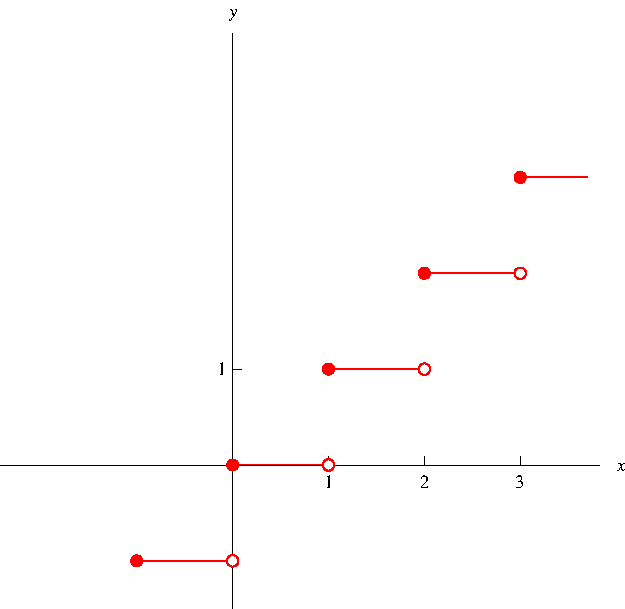
\includegraphics[height=4.5cm]{continuity/pictures/02-05-ex2d.pdf}%
\column{.6\textwidth}
\begin{itemize}
\item<2-| alert@3-4>  $f(n) = $ \uncover<4->{$n$.}
\item<2-| alert@5-6>  $\lim_{x\rightarrow n^+} f(x) = $ \uncover<6->{$n$.}
\item<7->  Continuous from the right at $n$.
\item<2-| alert@8-9>  $\lim_{x\rightarrow n^-} f(x) = $ \uncover<9->{$n-1$.}
\item<10->  Discontinuous from the left at $n$.
\end{itemize}
\end{columns}
\end{example}
\end{frame}
% end module continuity-ex3
